\documentclass[tikz,border=2pt]{standalone}
\usepackage{helvet}
\renewcommand{\familydefault}{\sfdefault}
\usetikzlibrary{positioning,arrows.meta,fit}
\definecolor{frozen}{HTML}{E6E6E6}
\definecolor{train}{HTML}{F6C77A}
\begin{document}
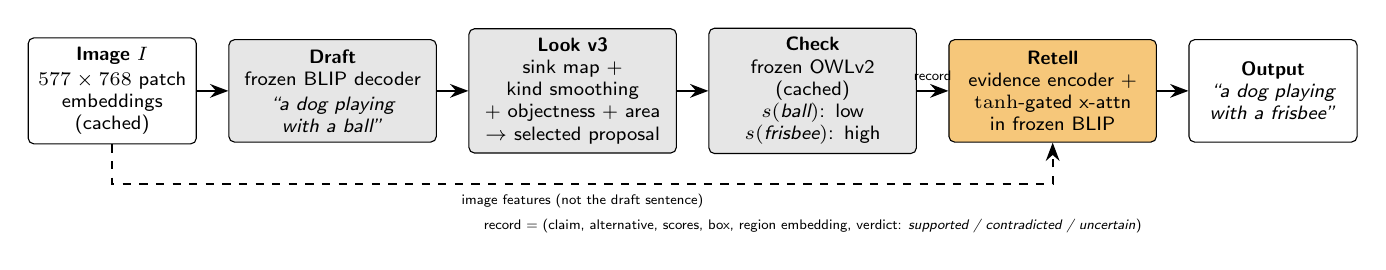
\begin{tikzpicture}[
  font=\scriptsize, >=Stealth, node distance=4mm,
  box/.style={draw, rounded corners=2pt, align=center, minimum height=13mm, text width=24mm, fill=frozen},
  tbox/.style={box, fill=train},
  io/.style={draw, rounded corners=2pt, align=center, minimum height=13mm, text width=19mm, fill=white},
  arr/.style={->, thick}]
\node[io] (img) {\textbf{Image $I$}\\[1pt]$577\times768$ patch\\embeddings (cached)};
\node[box, right=of img] (draft) {\textbf{Draft}\\frozen BLIP decoder\\[1pt]\emph{``a dog playing}\\\emph{with a ball''}};
\node[box, right=of draft] (look) {\textbf{Look v3}\\sink map + kind smoothing\\+ objectness + area\\$\to$ selected proposal};
\node[box, right=of look] (check) {\textbf{Check}\\frozen OWLv2 (cached)\\$s(\textit{ball})$: low\\$s(\textit{frisbee})$: high};
\node[tbox, right=of check] (retell) {\textbf{Retell}\\evidence encoder +\\$\tanh$-gated x-attn\\in frozen BLIP};
\node[io, right=of retell] (out) {\textbf{Output}\\\emph{``a dog playing}\\\emph{with a frisbee''}};
\draw[arr] (img) -- (draft);
\draw[arr] (draft) -- (look);
\draw[arr] (look) -- (check);
\draw[arr] (check) -- node[above, font=\tiny]{record} (retell);
\draw[arr] (retell) -- (out);
\draw[arr, dashed] (img.south) |- ++(0,-5mm) -| node[pos=0.25, below, font=\tiny]{image features (not the draft sentence)} (retell.south);
\node[below=7mm of check, font=\tiny, align=center] (rec) {record = (claim, alternative, scores, box, region embedding, verdict:
\emph{supported / contradicted / uncertain})};
\end{tikzpicture}
\end{document}
